% Definitions
\newcommand\wtfgenes{WTFgenes}

% Abstract
\structabs{
A common technique for interpreting experimentally-identified lists of genes
is to look for enrichment of genes associated to particular Gene Ontology terms.
The most common technique uses the hypergeometric distribution;
more recently, a model-based approach was proposed.
These approaches must typically be run using downloaded software, or on a server.
}{
We develop a collapsed likelihood for model-based gene set analysis and present \wtfgenes, an implementation of both hypergeometric and model-based
approaches, that can be published as a static
site with computation run in JavaScript on the user's web browser client.
Apart from hosting, zero server resources are required: the site can (for example) be served
directly from an S3 bucket.
A C++11 implementation yielding identical results runs roughly twice as fast as the JavaScript version.
}{
\wtfgenes\ is available from \url{https://github.com/evoldoers/wtfgenes}.
}{
Ian Holmes {\tt ihholmes+wtfgenes@gmail.com}.
}{
None.
}

\section*{Introduction}

Gene Set Enrichment Analysis (GSEA) \citep{pmid16199517}
Standard approach is a one-tailed Fisher's Exact Test (based on the hypergeometric distribution), with a correction for multiple hypothesis testing.
Numerous implementations e.g. GO::TermFinder \citep{pmid15297299}

Model-based Gene Set Analysis (MGSA) \citep{pmid20172960}
Bioconductor \citep{pmid21561920}

builds on earlier generative model by \cite{pmid18676451}

% description of MGSA from Bauer et al 2010

\begin{figure}
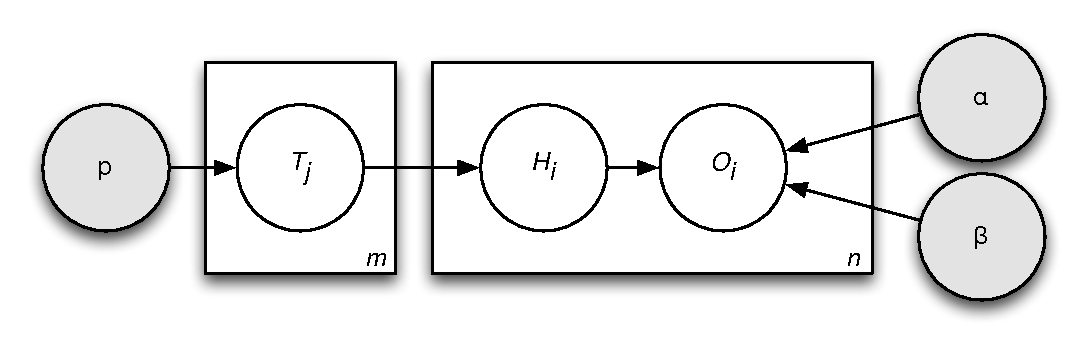
\includegraphics[width=\columnwidth]{model}
\caption{
  \label{fig:model}
  Model-based explanation of observed genes ($O_j$) using ontology terms ($T_i$), following \cite{pmid20172960}.
}
\end{figure}

The MGSA model is sketched in Figure~\ref{fig:model}.
For each of the $m$ terms there
is a boolean random variable
$T_j$ (``term $j$ is activated'').
For each of the $n$ genes there is a directly-observed boolean random variable
$O_i$ (``gene $i$ is observed in the gene set''),
and one deterministic boolean variable
$H_i$ (``gene $i$ is activated'')
defined by $H_i = 1 - \prod_{j \in G_i} T_j$
where $G_i$ is the set of terms associated with gene $i$
(including directly annotated terms, as well as ancestral terms implied by transitive closure of the directly annotated terms).
The probability parameters are $\pi$ (term activation), $\alpha$ (false positive) and $\beta$ (false negative),
and the respective hyperparameters are ${\bf p}=(p_0,p_1)$, ${\bf a}=(a_0,a_1)$ and ${\bf b}=(b_0,b_1)$.
The model is
\begin{eqnarray*}
P(T_j=1|\pi) & = & \pi \\
P(O_i=1|H_i=0,\alpha) & = & \alpha \\
P(O_i=1|H_i=1,\beta) & = & 1-\beta
\end{eqnarray*}
with
$\pi \sim \mbox{Beta}({\bf p})$,
$\alpha \sim \mbox{Beta}({\bf a})$ and
$\beta \sim \mbox{Beta}({\bf b})$.
The model of \cite{pmid20172960} is similar but used an
{\em ad hoc} discretized prior for $\pi$, $\alpha$ and $\beta$.

Most MGSA and GSEA implementations are designed for desktop use.

Several GSEA implementations are designed for web use, notably Enrichr \citep{pmid23586463,pmid25971742,pmid27141961}
which has a rich dynamic web front-end.
However these web-facing GSEA implementations generally require a server-hosted back end.
Further, there are no web-based MGSA implementations.

\section*{Results}

We sample from a collapsed version of the MGSA model in Figure~\ref{fig:model} by integrating out the probability parameters.
Let $c_p = \sum_j^m T_j$ count the number of activated terms,
$c_g = \sum_i^n H_i$ the activated genes,
$c_a = \sum_i^n O_i(1-H_i)$ the false positives and
$c_b = \sum_i^n O_i H_i$ the false negatives.
Then
\[
P({\bf T},{\bf O}|{\bf a},{\bf b},{\bf p}) =
Z(c_p;m,{\bf p})
Z(c_a;n-c_g,{\bf a})
Z(c_b;c_g,{\bf b})
\]
where
\[
Z(k;N,{\bf A}) =
\left( \begin{array}{c} N \\ k \end{array} \right)
\frac{B(k+A_0,N-k+A_1)}{B(A_0,A_1)}
\]
is the beta-binomial distribution for $k$ successes in $N$ trials with pseudocounts ${\bf A}=(A_0,A_1)$,
using the beta function
\[
B(x,y) = \int_0^1 t^{x-1}(1-t)^{y-1} dt = \frac{\Gamma(x)\Gamma(y)}{\Gamma(x+y)}
\]
Integrating out probability parameters improves sampling efficiency
and allows for higher-dimensional models where, for example, we observe multiple gene sets
and give each term its own probability $\pi_j$
or each gene its own error rates $(\alpha_i, \beta_i)$.
Our implementation by default uses uninformative priors with hyperparameters ${\bf a}={\bf b}={\bf p}=(1,1)$
but this can be overridden by the user.

The MCMC sampler uses a Metropolis-Hastings kernel where each proposed move perturbs some subset of the term variables.
These moves include {\em flip}, where a single term is toggled;
{\em step}, where any activated term and any one of its unactivated ancestors or descendants are toggled;
{\em jump}, where any activated term and any unactivated term are toggled; and
{\em randomize}, where all term variables are uniformly randomized.
The relative rates of these moves can be set by the user.

The sampler of \cite{pmid20172960} implemented only the {\em flip} move.
To test the relative efficacy of the newly-introduced moves we measured the autocorrelation of the term variables
for one of the GO Project's test sets, containing 17 {\em S.cerevisiae} mating genes.
\footnote{Gene IDs: STE2, STE3, STE5, GPA1, SST2, STE11, STE50, STE20, STE4, STE18, FUS3, KSS1, PTP2, MSG5, DIG1, DIG2, STE12.}
The results, shown in Figure~\ref{fig:termauto}, led us to set the MCMC defaults such that
the {\em flip}, {\em step}, and {\em jump} moves are equiprobable,
while {\em randomize} is disabled.

\begin{figure}
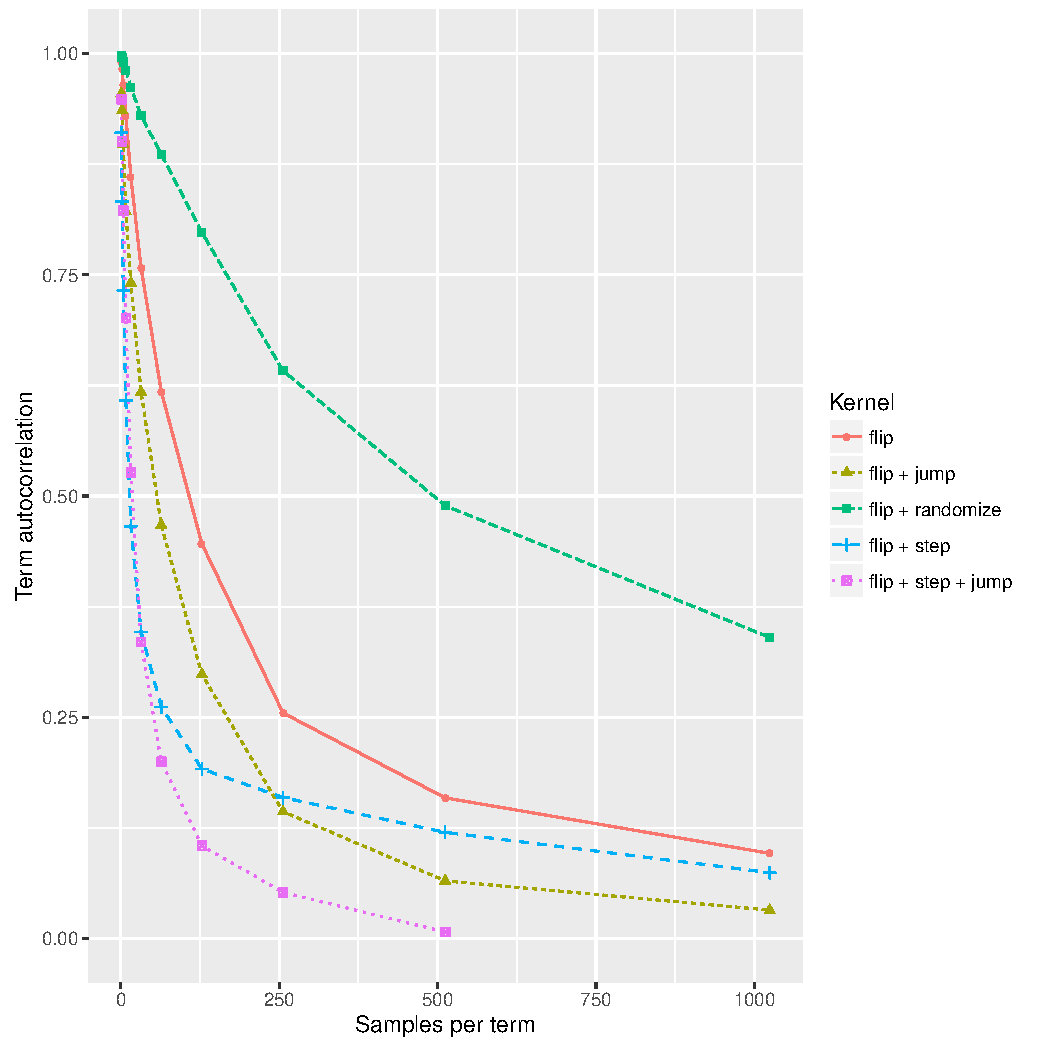
\includegraphics[width=\columnwidth]{termAutoCorrelation}
\caption{
  \label{fig:termauto}
  Autocorrelation of term variables, as a function of the number of MCMC samples, for several MCMC kernels on a set of 17 {\em S.cerevisiae} mating genes.
  A rapidly-decaying curve indicates an efficiently-mixing kernel.
}
\end{figure}

We have implemented both GSEA (with Bonferroni correction) and MGSA (as described above), in both C++11 and JavaScript.
The JavaScript version can be run as a command-line tool using node, or via a web interface in a browser, and includes extensive unit tests.
The two implementations use the same random number generator and yield numerically identical results.
The C++ version is about twice as fast:
a benchmark of MGSA on a late-2014 iMac (4GHz Intel Core i7),
using the abovementioned 17 yeast mating genes and the relevant subset of 518 GO terms, run for 1,000 samples per term,
took 37.6 seconds of user time for the C++ implementation and 79.8 seconds in JavaScript.
By contrast, the GSEA approach is almost instant,
though less statistically powerful than MGSA if the observed gene set is indeed generated by a small number of terms \citep{pmid20172960}.

When run via a web browser, the JavaScript implementation can be deployed as a ``static site'',
i.e. consisting only of static files (HTML, CSS, JSON, and JavaScript) that can be hosted via a minimal web server with no need for dynamic code execution.
This has considerable advantages: static web hosting is generally much cheaper, and far more secure, than running server-hosted web applications.

\section*{Discussion}

JavaScript genome browsers such as JBrowse \citep{pmid27072794}
are consistent with a broader web trend of producing static sites where possible

Not a direct competitor to Enrichr, which has much richer visualizations and allows user submission of gene sets,
consequently requiring a server back-end

The model-based approach is versatile: it can readily be extended
to applications that are structured
temporally \citep{pmid26111374},
spatially \citep{pmid26877824},
by genomic region \citep{pmid20436461},
or using domain-specific biological knowledge \citep{pmid24675718}.


\section*{Funding}

IHH was partially supported by NHGRI grant R01-HG004483.

\bibliographystyle{natbib}
%\bibliographystyle{bioinformatics}
%\bibliographystyle{achemnat}
%\bibliographystyle{plainnat}
%\bibliographystyle{abbrv}
%
%\bibliographystyle{plain}
%
%\bibliography{Document}


\bibliography{references}
